% REMEMBER: You must not plagiarise anything in your report. Be extremely careful.

\documentclass{l4proj}
\usepackage{algorithm2e}
%
% put any additional packages here
%

\begin{document}

%==============================================================================
%% METADATA
\title{Accelerating Spaceship Search Using Deep Learning in John Conway's Game of Life}
\author{Paul Bekaert}
\date{October 7, 2022}

\maketitle

%==============================================================================
%% ABSTRACT
\begin{abstract}
    \vskip 0.5em
    ``John Conway's game of life is a widely known cellular automaton which gives rise to interesting structures. One of these structures are spaceships, which move with a constant speed in one direction. Conventional spaceship search algorithm in the game of life tend to be slow due to the discrete nature of the task, and the number of possible cell combinations. In this paper, we investigate the possibility of speeding up spaceship search by using a neural network to predict cells that are in a ship. The search is implemented in an A* type fashion, with one network predicting the leaf nodes, and the other implementing a heuristic function. This is a difficult task as the game of life is inherently deterministic, and training a network for this problem would be an interesting development in finding patterns in other cellular automata. It was found that the search method implemented has difficulty converging onto a solution with spaceships that have not been used as training data, most likely due to a lack of enough spaceship data. However, the heuristic function worked surprisingly well in predicting the distance to a potential spaceship.''
\end{abstract}

%==============================================================================

% EDUCATION REUSE CONSENT FORM
% If you consent to your project being shown to future students for educational purposes
% then insert your name and the date below to  sign the education use form that appears in the front of the document. 
% You must explicitly give consent if you wish to do so.
% If you sign, your project may be included in the Hall of Fame if it scores particularly highly.
%
% Please note that you are under no obligation to sign 
% this declaration, but doing so would help future students.
%
\def\consentname {Paul Bekaert} % your full name
\def\consentdate {7 October 2022} % the date you agree
%
\educationalconsent


%==============================================================================
\tableofcontents

%==============================================================================
%% Notes on formatting
%==============================================================================
% The first page, abstract and table of contents are numbered using Roman numerals and are not
% included in the page count. 
%
% From now on pages are numbered
% using Arabic numerals. Therefore, immediately after the first call to \chapter we need the call
% \pagenumbering{arabic} and this should be called once only in the document. 
%
% Do not alter the bibliography style.
%
% The first Chapter should then be on page 1. You are allowed 40 pages for a 40 credit project and 30 pages for a 
% 20 credit report. This includes everything numbered in Arabic numerals (excluding front matter) up
% to but excluding the appendices and bibliography.
%
% You must not alter text size (it is currently 10pt) or alter margins or spacing.
%
%
%==================================================================================================================================
%
% IMPORTANT
% The chapter headings here are **suggestions**. You don't have to follow this model if
% it doesn't fit your project. Every project should have an introduction and conclusion,
% however. 
%
%==================================================================================================================================
\chapter{Introduction}

% reset page numbering. Don't remove this!
\pagenumbering{arabic} 

\section{Motivation}

[REFERENCE THIS]

The game of life (GoL) has often been seen as a toy project. It is idealistic in its representation, as it is fully observable, episodic and deterministic. However, its simple rules give rise to complex structures that are not easy to find. Those structures can be arbitrarily large, and looking for ships above a width and height of $100 \times 100$ is close to unfeasible with current methods. In general, conventional graph search methods adapted to the task are are used to find said structures. \cite{list_of_search_algorithms}. There is still a lot of room for improvement for these algorithms, and optimizing the search is still an open issue.

The concept of using deep learning to find structures in cellular automata has not yet been explored. With the advent and rise of neural networks, previously thought to be impossible problems have been unlocked, either by solving them directly or speeding up existing algorithms. Since this is a difficult search problem, it stands to reason that solving it will potentially give new insights into how to solve similar problems in cellular automata.


% MAKE THE AIMS MORE CLEAR
\section{Aims}

In this paper, we will be trying to find interesting structures in the game of life. Our particular interest will be in oscillating objects that move a set amount of space, so-called 'spaceships'. The main goal will be to test and see if neural networks can speed up the search, and how different deep learning techniques fare against each other and other conventional search methods. The expectation is that the network will greatly decrease the time it takes to find novel structures or structures already classified as spaceships.

% CHECK THIS 30 VALUE
This search algorithm is especially challenging to implement due to the aforementioned deterministic nature of the problem. There are $2^{w * h}$ possible structures in a given grid of width and height $w$ and $h$ respectively, from which only $\sim{30}$ structures known structures exist. It also bases the functionality of the algorithm on a single hypothesis that is tested in this paper. 

%==================================================================================================================================

\chapter{Background}

\section{The game of life}
% ========

\subsection{Rules}

"The Game of Life" is a zero-player game (a simulation of sorts) invented by John Conway in 1970 which describes a cellular automata (CA) with a set of rules. A cellular automata is a simulation of cells evolving every time step, which are represented in a matrix of size $n\times m$. Every time step, the cells are modified using a set of pre-defined rules. In John Conway's Game of life (GoL), a cell is either dead or alive, represented as a $0$ or a $1$ respectively. The neighbourhood of the cell is defined as Moore's neighbourhood, which is the 8 cells adjacent to the cell, diagonally and orthogonally. It can also be thought of as a $3\times 3$ matrix where the subject cell is placed in the middle. The number of neighbours the cell has is the number of cells alive that are present in the cell's Moore neighbourhood, $n$. We can then define the rules of the CA described in Life:

\begin{itemize}
    \item A dead cell turns into a living cell if $n \geq 3$
    \item A dead cell stays dead if $n < 3$
    \item A living cell stays alive if $n = 2$ or $n = 3$
    \item A living cell dies if $n < 2$, due to under-population
    \item A living cell dies if $n > 3$, due to overcrowding
\end{itemize}

A state at $t+1$ is entirely dependant on the current state at $t$ and is calculated using the rules above. The game can go on indefinitely, but usually reaches a state in which cell structure does not change in any significant way. For example, all the cells could die, creating an empty board. More likely however, is that the resulting state will be populated with still-lifes, oscillators, and sometimes spaceships, which are defined below.

\begin{figure}[h]
\centering
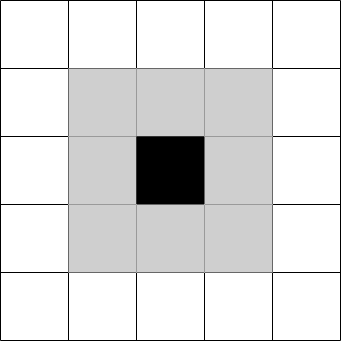
\includegraphics[width=0.4\linewidth]{dissertation/images/diagrams/moores_neighbourhood.png}
\caption{Moore's Neighbourhood. This is the space of interest for any given cell (grey squares). The number of neighbours a cell has is the number of alive cells within this neighbourhood.}
\label{fig:subim1}

\end{figure}

\subsection{Still lifes}

A still life is a structure that does not move or change shape from generation to generation. They remain static (do not move around the board or in shape), unless outside cells interact with it. Still lifes are by far the most common structures in the GoL, and they are easy to find, as they have the same shape for $t$ and $t+1$. Here are some examples of still lifes:

\begin{figure}[h]
\centering
\begin{subfigure}[b]{0.2\textwidth}
    
\includegraphics[width=\textwidth]{dissertation/images/gol_structures/still_life_1.png} 
    \caption{The Block} %SHOULD I GET RID OF THIS ONE OR RE-DRAW IT SOMEHOW?
    \label{fig:subim1}
\end{subfigure}
\hfill
\begin{subfigure}[b]{0.2\textwidth}
    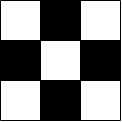
\includegraphics[width=\textwidth]{dissertation/images/gol_structures/still_life_2.png} 
    \caption{The Tub}
    \label{fig:subim1}
\end{subfigure}
\hfill
\begin{subfigure}[b]{0.2\textwidth}
    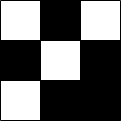
\includegraphics[width=\textwidth]{dissertation/images/gol_structures/still_life_3.png} 
    \caption{The Boat}
    \label{fig:subim1}
\end{subfigure}

\caption{Examples of still lifes}
\end{figure}

\subsection{Oscillators}

These are structures that change shape, but return to the same state every $p$ generations. They are  harder to detect, as it is impossible to know how many generations it will take for the structure to repeat. An oscillator will stay in the same position after it has oscillated, and will keep oscillating as long as it is undisturbed by other cells and the program keeps running. Here are some examples of oscillators:

\begin{figure}[h]
\centering
\begin{subfigure}[b]{0.4\textwidth}
    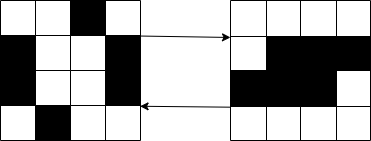
\includegraphics[width=\textwidth]{dissertation/images/gol_structures/toad_transition.png} 
    \caption{The Toad}
    \label{fig:subim1}
\end{subfigure}
\hfill
\begin{subfigure}[b]{0.4\textwidth}
    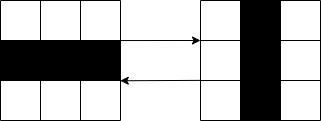
\includegraphics[width=\textwidth]{dissertation/images/gol_structures/blinker_transition.png} 
    \caption{The Blinker}
    \label{fig:subim1}
\end{subfigure}

\caption{Examples of oscillators and their different iterations}
\end{figure}

\subsection{Spaceships}

% TALK MORE ABOUT THEM
Spaceships are the main focus of this paper, and are the hardest structures to detect. They are similar to oscillators in that they repeat their state every $p$ generations. However, they also move a certain distance since their last oscillation. If the state space they are in is unbounded, then they will move forever without changing direction.

The speed of a spaceship is determined in terms of the speed of light of GoL, $c$. This $c$ is defined as 1 cell per second, as it is theoretically the quickest information could hope to propagate given the rules of Life. The ship can move diagonally, orthogonally, or knightwise, which is when a ship moves in an oblique direction. A spaceship with a period $p$, which is moving $n$ cells in a particular direction is said to have a speed $nc/p$. A ship moving $n = 2$ cells left and with a period $p = 5$ will have a speed of $2c/5$. For a ship moving knightwise $n$ cells either left or right, and $m$ cells either up or down, will have a speed denoted as $(m, n)c/p$. These speeds can be simplified, for example a spaceship moving at speed $2c/4$ can be written as $c/2$.

\begin{figure}[h]
\centering
\begin{subfigure}[b]{0.3\textwidth}
    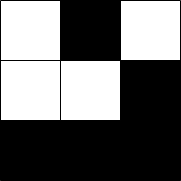
\includegraphics[width=\textwidth]{dissertation/images/gol_structures/glider.png} 
    \caption{The glider}
    \label{fig:subim1}
\end{subfigure}
\hfill
\begin{subfigure}[b]{0.3\textwidth}
    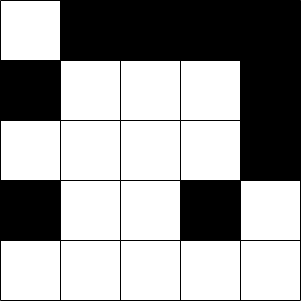
\includegraphics[width=\textwidth]{dissertation/images/gol_structures/LWSS.png} 
    \caption{The LWSS}
    \label{fig:subim1}
\end{subfigure}

\caption{Examples of spaceships}
\end{figure}

There are 2 principle ways of classifying spaceships: engineered and elementary ships. Elementary spaceships are those which can be found naturally in the GoL via searching a random soup, which is starting with a random grid of cells and it evolving into a spaceship They are also classified as ships that have been found by a search algorithm. Engineered spaceships are those created by people using small interacting parts to assemble a ship as a whole. There are an infinite amount of spaceships in the GoL, however few elementary spaceships have been found, whilst some engineered spaceships have been found that can be extended forever. In this paper, a mix of engineered and elementary spaceships are used as test data, and the search looks for both equally.

% ========

\section{Different ways to find spaceships}

The problem we're trying to solve is to new spaceships in general, however the focus are on "interesting" ships, which consist of mostly elementary ships, and some engineered ones. These are, as explained above, structures that repeat inside of a game of life grid, but also move a certain amount of space. This is a widely known toy problem, however it is an NP-hard problem, which means brute force is out of the question. In a given $n \times m$ grid, there are $2^{n \times m}$ possible combinations. For example, a glider, which takes at least a $3x3$ grid to be represented, would be found by searching $2^{9}$ grids. Brute force becomes unfeasible after approximately $n > 6, m > 6$. This algorithm tends not to have much use, but it has found a comprehensive list of all still-lives, oscillators, and spaceships within a small rectangle.

A better approach is representing the board as a graph. By representing each cell as a path- a path where the cell is either alive or a path where the cell is dead- a tree search method can be used. This is the method used in most algorithms today, by trying to optimize which cell should be placed next. Some combinations of cells should not be placed together as the result would be incompatible with a spaceship, and therefore the algorithm can eliminate entire sub-trees from the search space.

\section{Existing Search Methods}

There are not many research papers on the subjects, but in Searching for Spaceships \cite{searching_for_spaceships}, a de Bruijn graph is used to represent the cells. The algorithm - "gfind" - only works on one side of the ship, and assumes the other to be symmetrical. A ship is then constructed by applying the GoL rules to rows of the ship, and placing the formed cell in front of the ship in the direction it will move. To visualize this, imagine the grid follows the ship as it is moving, so that the ship looks like it is simply oscillating. A future oscillation can therefore be predicted by taking the evolution of the spaceship for every row of 3, and applying it $p$ (the speed of the ship) cells above the evolution, as it would reach that point p next iteration. This approach has one major drawback- any spaceship that is not a "long" spaceship will not be detected. The search space also does not include asymmetrical spaceships, of which there are many.

Another well known algorithm to find spaceships or oscillators is "lifesrc" created by David Bell, uses a depth first backtracking search. The grid is first set up with a few 'known' cells, set by the user. The rest of the cells are classed as 'unknown'. When the algorithm starts running, a decision is made on whether a cell should be alive or not, and the program will check forward and backward if there are any oscillating patterns of period $p$ set by the user. If nothing is found, the search continues, using the decided cell. If it is found later on that a cell placement in a particular cell is impossible, or that there are no oscillators in a particular configuration, then the algorithm will backtrack to the latest cell it decided on randomly. This is essentially a depth first search, however it discards certain sub-trees by eliminating ones that do not follow the Life rules (for example, checking if every cell is alive in a $4 \times 4$ grid would be redundant, since almost all cells in that grid would die in the next iteration). 

The most efficient algorithm used to find spaceships today is dubbed the 'ikpx2' algorithm, which was created by Adam P. Goucher. It was inspired by gfind, which searches De Bruijn graphs representing the different parts of a spaceship. However, ikpx reduces the spaceship search problem into a set of SAT constraints, which can then be used on an SAT solver. The problem is reduced to by using quotient latices to represent cell structure, and cell combinations which cannot exist together are false, whilst possible patterns are set to true. The solver used in question is the "iglucose" \cite{sat_2018} SAT solver and sped up the search considerably, as a lot of research has gone into accelerating SAT solvers. A notable find by the ikpx2 algorith was the 'knightship': the first oblique spaceship found, or in other words, a spaceships that does not move diagonally nor orthogonally. This reduction to SAT also proves that the search method is at least NP-complete, which is a difficult problem to solve.
[IS THAT CORRECT]

\section{Deep Learning with the GoL in General}

There are a few research papers written on neural networks and the game of life, with one notable one being about forward planning in the GoL \cite{game_of_life_dl_is_hard}. In this paper, they try to predict the future structure of a starting configuration. They used several 1x1 and 3x3 convolutional layers in their network, activated by ReLU functions. Although the model was able to perfectly predict the next iteration of the game, the further the model tries to predict, the worse the result. The problem hypothesised by Springer is the 'lottery ticket problem', in which the starting configuration of the model is what would allow it to converge to a correct solution. 

Apart from research done, there are many hobbyists working on combining deep learning with GoL. One of them is James McGuigan, who trained a neural network to learn the game of life after one iteration. He has also worked on reversing the game of life, trying to find a previous configuration using a current board state. Another notable use of deep learning and the game of life is by NeatAI, who used genetic algorithms in the game of life \cite{neatai_gol}. He used a $c$ function that calculates the overall 'complexity' of the current structures in the grid. For example, a grid with random cells is not very interesting, but one that has a couple of gliders and oscillators with high periods may be of more interest. To design his $c£$ function, he took inspiration from a paper by \cite{algorithmic_specified_complexity}, which describes a process of encoding interesting objects in the game of life. It uses features of an object such as shift, repeating period, intersection between 2 or more objects, to define the properties of such an object, These properties are then bit-encoded to form a number that specifies the complexity of the object. To find the complexity of a particular state on a board, the sum of the object complexities is taken.

NeatAI took this $c$ function and applied it to a neural network which determined whether or not a cell should be alive given the input parameters $x$, $y$, population density, and bias. He then used genetic neural networks to improve his model to maximize the $c$ function. The net improved by making optimal start configurations for the model to evolve into. This is an interesting concept, as if the $c$ function were to be changed to be maximised by how far a pattern has reached from the origin, it could potentially be used to find new spaceships for example.

\section{Summary}

In this section, we've defined the game of life and its rules set by John Conway. This involved the definition of a cellular automata, the way the board evolves over time, Moore's neighbourhood, and the rules for a cell to be dead or alive. Different definitions of structures were shown, such as still lifes like the block, or oscillators like the blinker. Spaceships were defined as an interesting oscillating structure that moves across the board with a certain speed which can be denoted using the "GoL speed of light", $c$, which is the maximum speed information can propagate (1 cell per iteration). We then looked at different ways to find spaceship, namely brute force (which is computationally impossible after a certain point due to to the NP hardness of the problem) and tree search. Tree search involves representing cell changes as nodes on a tree, and searching the tree for a solution. Existing search methods were covered such as "ikpx" and "gfind". Their use of de Brujin graps- and SAT solvers for "ikpx"- was detailed, again using tree search to find structures. Finally, an overview of deep learning in the game of life was mentioned. Although there has not been much research done in this field, there have been amateurs working on it such as James McGuigan, who tries to train neural networks into learning the previous state of any given state. Furthermore, others have tried to simulate a GoL state after $k$ steps, with limited success.

%==================================================================================================================================
\chapter{Design}

\section{The Problem To Solve}

The main objective of this paper is accelerating tree search of spaceships in the game of life by using neural networks. The search method will follow an A* search pattern, wherein a scoring network will be used as a heuristic function, and a probability change network will be used to select which cells should be used as branches. This network is responsible for scoring potential cells to be changed in a given structure. The algorithm then uses threshold values to find which cells should be added as a branch to the current state. These branches are then scored by the heuristic function. The networks will be trained on spaceships only below the size of $100 \times 100$, however in theory, the network could then work for any size.

\section{The Main Assumption}

Neural networks can be good at detecting general patterns in objects. There has been a lot of debate in the GoL community about an underlying pattern to spaceships. There have been methods by the community which use "spaceship engineering" - combining multiple identified sub-parts of spaceships to make a new moving ship. However, there has yet to be a formalized equation or pattern found to help fast-track the search of such ships. To use a neural network for this problem, the approach taken in this paper revolves around the assumption that spaceships have an underlying pattern which is detectable to a neural network. Although there are not many spaceships, data expansion methods are used to gather more data, and convolutional techniques are used to train the network. This assumption is also used in the scoring network, as only ships that have been trained on will have a high score, implying that there is also some type of general pattern. 


\section{The Search Algorithm}

The algorithm is a standard A* tree search, but uses two neural networks to help accelerate it. The first network is trained to generate branches for any given node, and the second is used as a heuristic function. Every node in the tree contains a grid, which is the state of a GoL world, and a number of times it has been visited. The branches of the node represent a change of 1 cell from that node. For example, a cell that has been brought to life, or a cell that has been killed. The first network outputs a probability change grid for every cell in said grid. This probability change is how much the network believes the cell should change. If the probability is near 0, then the cell should stay unchanged. However the closer to -1 or 1 the probability change value is, the more probable that it must be changed. Branches of the current node are based off this probability change output, which is first filtered via thresholds, and then changes with the biggest magnitude are used as branches. The top $n$ cells with the greatest magnitude of change are then used to create $n$ new grids with that change taken into account. Then, the algorithm scores these new grids using the scoring neural network. This is used as a heurstic function to find the grid which is most likely to converge to a spaceship. The heuristic function is combined with the number of times a node is visited, which allows search of the entire tree structure and prevents loops.  

said branches by taking the top $n$ cells with the greatest probability change. 
. This will then be used in a tree search algorithm, with branches generated given the highest changes in probability. The second network is trained to predict the mean square error of a given configuration. This is to be used as a heuristic for the A* algorithm.

The probability prediction network receives as input a grid of arbitrary size with probability values between 0 and 1. The network will then predict a change in probability grid. The highest changes in probability (positive or negative) are then applied to a new grid. these grids then become the branches of a node. Using the scoring network, the grid with the lowest score is then chosen to be the next node. This is effectively an A* search technique.

\section{The Networks}

There are two main networks that this algorithm will use to guide the search:

\begin{itemize}
    \item The probability network: used to find which cells should be modified
    \item The scoring network: used as a heuristic function
\end{itemize}

The probability network uses a fully convolutional network without pooling layers. Swish activation functions are used between each convolution, and will output a convolution that retains the size of the input. Input of the network consists of a configuration of cells with values ranging from 0 to 1, each representing a probability of a cell being present. The output is then given as a change of probability of the input.

The scoring network also uses a series of convolutions, but is then followed by an average pooling layer, and finally a fully connected layer to predict a final score between 0 and 1. Scoring of this network is used as a heuristic to find how far a given solution is from converging towards a spaceship; the idea being that this problem can be turned into an A* type of search.

\section{Data used to train the network}

For a ship to qualify as a training item in the network, it needed to be under $100 \times 100$ in width and height. This is done for data processing reasons: creating and augmenting the data at greater sizes than this will be significantly slower. The ships selected were all different in structure. That is, any spaceship was independent; for example, an engineered spaceship that is infinitely extendable would only appear in the dataset in its minimum size (minimum working form). A majority of the spaceships used in the dataset were elementary ships for this reason.

One major problem with training the networks is the lack of enough spaceship data. There are not many spaceships which follow different patterns known in the game of life. This leads to the networks learning a specific ship pattern, instead of a general structure for these ships. In order to mitigate this problem, data augmentation was performed. A ship is evolved through all of its different shapes until reaching its original structure. This gives $p$ more grids to train with, where $p$ is the period of the ship this method is being applied to. Once that step is complete, further augmentation can be done by rotating the ship in all 4 directions. Since the GoL rules are the same in every direction, this will not break the spaceship. Using this method, it was possible to enlarge a dataset of $\sim 30$ ships into $\sim 900$ ships.

To get the necessary data to train the actual networks, input-target pairs were needed. These were obtained by removing a number of cells from a spaceship, and adding a number of cells to other parts of the ship that weren't there originally. This had the effect of creating a li+++near path of reconstruction given a starting grid of cells. The number of missing and added cells was increased linearly, and the number of added cells was also randomized to add some noise, preventing the neural network from learning to base a ship on the number of cells alive. A solution matrix can then be constructed by taking the difference between the actual ship and the deconstructed grid. The probability network used the deconstructed grid as input, and the solution grid as an output, since its target is the solution matrix. As for the scoring network, an MSE (Mean Squared Error) function can be used to evaluate the MSE between the original ship and the deconstructed version. This score can then be used as a training value for the network. 

\section{Summary}

The design section begins with an explanation of the main features of the algorithm, including a short description of tree search. Nodes are used to represent a particular board, and the networks are applied to these boards. The probability system was also explained, wherein the cell probabilities are used to chose which cells will be switched next. The probability change network was detailed, talking about how candidate cells are extracted from this probability network, and then scored by the scoring network. The main assumption for this to work is addressed, that being that an underlying general pattern must exist in GoL spaceships. Finally, data extraction: which spaceships were included, how to extract more spaceship data from any singular ship, and the training data that can be created with the deconstruction method. The deconstruction method was talked about in detail, as it was used to train the networks used in the algorithm.


%==================================================================================================================================
\chapter{Implementation}

\begin{figure}[h!]
\centering
\includegraphics[width=\textwidth]{dissertation/images/diagrams/general_structure.jpg} 
\caption{General structure of the implementation of the search algorithm. This includes data, training models, the search itself, and tools.}
\label{fig:subim1}
\end{figure}

\section{Software Engineering Practices}

Identifying what needed to be done in the project was key to advancing in a timely manner. To do this, I kept an organised file which contained the tasks and objectives of the project, and a set list of things I needed to do within a certain week. In addition to this, I used the waterfall project development method, which suited the project well as it was a clear incremental step-based approach: first design a network to predict good cell probability values, then create a scoring network, and then assemble everything. Each step of the process had to be tested individually and as a whole. I also kept a sheet logging the hours I put in the project, and what I did during those hours. GitHub was used as version control for the project, and to allow my supervisor to access my code easily.

\section {Unsuccessful Attempts}

In this section, alternative initial methods to find spaceships that were initially tried are explained. These methods did not work out for a variety of reasons, but helped pave the way to the current search algorithm. 

\subsection{Ship Probability}

My first try to solve this problem revolved over giving structures a "probability" as to how close they are to being a spaceship. The idea was to teach a network the probability of a structure being a ship. A series of convolutions and pooling was used, followed by an adaptive convolutional layer which was then fed to a fully connected network. Given an input, this network would produce a probability of the input being a spaceship. This technique did not work for several reasons: The pooling lost information about the structure, the fully connected network was not able to properly converge, and the output was a softmax which was unreliable as a probability. Furthermore, the training data used on this network was not as complete as the training data used in future trials. Instead of the deconstruction of ships as mentioned in section 4.3, the data it trained on was either a ship or a random collection of cells. There are multiple problem with this, but the main issue would be that a ship would have abundant amounts of dead cells around it, which made them easy to detect by the network. To counter this problem, different density ratios were used, along with reducing the size of the random noise to be that of the size of a spaceship. However, this did little to improve the network, most likely due to its fully connected nature, which failed to converge due to having to learn locality from scratch.

This probability prediction neural network was fed to a tree search which worked by flipping cells off and on and checking if the probability of the structure being a spaceship increased. This did not work very well, partially because the network did not produce good results, but also because the fully connected layer meant that changing a single cell did not change the final output significantly. Large changes in the structure did yield better results, since a greater change in the input would produce a change to the fully connected layer, but was ultimately not useful for finding new ships. 

This initial network may sound familiar: the scoring network used in the search algorithm. However, there is one key difference between the two. While the ship probability algorithm tried to find the \emph{probability} of a structure being a ship, the scoring model tries to model the \emph{positive MSE loss} of a structure to a spaceship. The positive MSE loss is essentially the same as MSE loss: however the higher the value the better the score. This scoring function is more reliable than a probability, as it best represents how 'close' the ship is to being complete, which is what the search algorithm converges towards.

\subsection {Stochastic Ship Cell Probability}

This second method attempted was similar to the method being used now. As mentioned, the value of every cell is represented as the probability of a cell being alive. This originally came from the idea that perhaps a stochastic version of the search algorithm could be used: activate cells based on the probability of them being alive, and then check if it is a spaceship. Repeat this until the probabilities are polarised to one side or the other. This did not work for a major reason: since the problem is deterministic, one small error in a cell can lead to the difference between a spaceship or not. With a stochastic search, even if the probabilities are close to being correct, the error in probability can quickly add up and reduce the chance of a spaceship being generated significantly. In addition to this, the network training did not fit well enough to be used in a probabilistic manner. Since the model was trained on 1s and 0s, applying the network output on itself would give the same exact output from the last iteration, which meant there was no change of input for the model. Furthermore, since there are on average a large amount of dead cells in any given spaceship, the model was trained to decrease probabilities everywhere. This means that after a few iterations, the probability of any cell was 0.
%This could have worked if more data was used, but the dataset used for the current search algorithm was already huge?

% REWRITE THIS
\section{Challenges faced}

Finding spaceships has been a challenge many in the GoL community have attempted, mostly using algorithmic methods and logical tree search programs. However, there is close to no research done on deep learning in the game of life, and no one has tried to find spaceships before. Researching the topic was not easy, and this made it very hard to base the program off previous research, which is why the resulting method is a tree search.

The search problem is NP-hard, so any conventional algorithm would be extremely slow in navigating the search space. The main aim of the paper is to accelerate this search using deep learning, but the problem remains very difficult, as a tree search approach is still used. 

Another issue was overfitting. It is very hard to get good results, and any that are found are most likely due to the network learning the spaceship structures instead of a general pattern, which is due to low diversity in spaceships. Even after data augmentation, the underlying spaceship pattern remains similar, and therefore may not be diverse enough. The original amount of spaceships used was $\sim 30$, which is a very low number.   

The amount of data available for training was problematic. As mentioned previously in section 3.4, there were not many spaceships to work with. Even if there exists a general pattern to spaceships as indicated in section 3.3, the lack of data may mean that this general pattern is impossible to identify due to the shortage of different types of ships. With more spaceships, a solution might be easier to converge on. However, using augmentation, a lot of extra data was created, even if still the same spaceship. The amount of augmented data used by this network was huge. Coupled with the fact that several convolutions are needed, training the network took days. Due to the limited time available, testing new networks was difficult, as training had to take place on another computer with a better GPU. This meant that even small changes to convolution size or other such parameters would take days to get results, and slowed down the testing process significantly. Hyper parameters might have been tuned to a better degree had there been a better way to train the networks.


\section{Probability Search}

\subsection{Choice of Technologies}

This project is the first time I ever used deep learning to complete a project, which meant I needed a quick and easy introduction into deep learning. The most obvious choice as someone who is good with Python and has never done any sort of machine learning was PyTorch. It allows for quick assembly of a neural network in python, and can be easily tested. Numpy was essential to allow rapid evaluation of GoL states. Since the code involves a lot of transformations of matrices, Numpy was perfect for quick and easy computation. Pandas and matplotlib were used heavily for the evaluation of my search method. Finally, to create a dynamic GoL testing environment, Pygame was used to represent the grid, iterate the matrix forwards/backwards, and generally see the results of search operations. Pygame was chosen for its simplicity when it comes to setting up a user interface, and even though it is slow, it was only used for data representation which made it ideal. If the matrix did not need to be interacted with, matplotlib was used. % EXPAND ON THIS IN THE FUTURE

\subsection{Data and Data Augmentation}

In this paper, the search is focused on elementary-like spaceships. Those are spaceships which are quite small (less than $100 \times 100$ in size), that have different speeds, and are usually elementary spaceships but there are a few engineered ships. These ships are classified as "interesting" by the community, and are stored in a database called "new-gliders.db" [CITE HERE]. The resulting dataset is quite small in size, fielding 31 spaceships in total. This is not ideal, as the number of ships should be as big as possible in order to get an idea of a ship pattern that will work well. To mitigate this lack of data, the ships were rotated to face all 4 directions, giving 124 different structures. Next, the ships were evolved in each direction, and all their period transitions were recorded. This expanded the dataset to around 1000 items.

\begin{figure}[h]
\centering
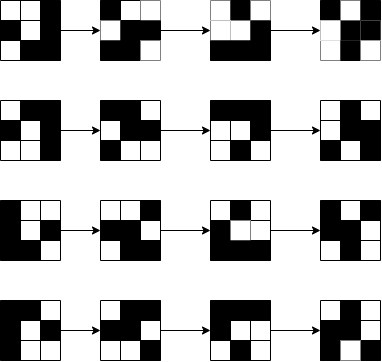
\includegraphics[width=\textwidth]{dissertation/images/diagrams/increasing_ship_data.png} 
\caption{Increasing dataset size by rotating ships in all 4 directions and iterating over all periods. Here you can see the Glider, which went from only 1 item in the dataset to 16.}
\label{fig:subim1}
\end{figure}

The next step of the process is to turn this ship into training data for the network. Several ideas were brainstormed, but the one that made the most sense is as follows: taking an initial spaceship, remove $n$ cells from this ship. At the same time, add a random number of cells sampled from a normal distribution around $n$ in locations where there should be none. Do this for different $n$ values, starting at 1 all the way to the number of cells the ship has. This does several things: it prevents the network from only learning where to place cells; as it also needs to remove them. It also does not let the network count the number of cells as the number of cells is random. This method of deconstruction yields a massive dataset. The final step is to give the network the "change in probability" values. Subtract the actual ship with the deconstructed matrix, and that gives the solution matrix for any given input. This data augmentation method can produce quite a lot of data, with parameters being the ratio of the ship to remove, and the number of cells to add to the structure.
% Maybe mention how this could produce different kind of results and maybe can be optimized to figure out almost completed ships, mid-range, and early range ships?

\begin{figure}[h]
\centering
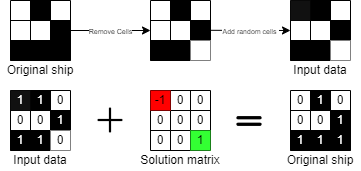
\includegraphics[width=\textwidth]{dissertation/images/diagrams/data_augmentation.png} 
\caption{Creating the input and solution matrices.}
\label{fig:subim1}
\end{figure}

The scoring network used similar data, however it needs to output a score instead of a matrix. The objective of the this network is to model the MSE (Mean Squared Error) between a ship and the structure. So, as a solution to a matrix, the MSE error is used as the target for the scoring network instead of a solution matrix. 

The data used in training the two networks were described generally in the design section of this paper. Mainly, expanding the dataset of known spaceships by iterating over all their possible states in any of the 4 directions (north, south, east and west, or more representatively, up, down, left and right). This is possible as for any structure in the GoL, it can be rotated $90^{\circ} $ without affecting its functionality. For example, a ship with period $p$, would therefore have $4 \times p$ valid spaceship states. For the Glider, which has $p = 4$, we can extract 16 configurations from only 1 valid one. Refer to Fig 3.1 in the design section for a graphic representation.

From the expanded dataset, more data can be created. The problem now is to create data that will be used to train our neural networks. Since the problem we are trying to solve is a change in probability given an input of living and dead cells, one approach is to show the network the solution matrix of a given configuration (Fig 3.2). This involves a deconstruction-reconstruction method. The method devised in this program was named $ratioDeconstruct()$, which took in a spaceship, and a ratio of the ship which should be deconstructed (0 being no deconstruction and 1 being deconstruction of the whole ship). A deconstruction ratio of 1 is recommended, as it allows the network to be exposed to entire ships as a solution. The ratio deconstruct method works as follows:

\begin{enumerate}
    \item Starting with a starting configuration, $x$, set a ratio of deconstruction $r$ and a number of configurations per deconstruction item, $n$. This $n$ value is the number of configurations generated for any number of missing cells in the ship.
    \item From this ratio and the number of alive cells in the spaceship, generate an array of all cell values that will be removed, $a$. This array can be generated by $i$ in $range(alive(x) \times r)$
    \item Once this array has been generated, loop over it. In a nested for loop, generate $n$ items as follows: Remove $i$ alive cells from the ship, which is the deconstruction part. Once deconstructed, generate a random number of alive cells calculated from a normal distribution centered on $i$, and add them to the original dead space of the ship. These are dummy cells, noise, added to the structure.
    \item Once the generated item has been created, $y$, create a solution matrix $s$ by $s = x - y$. A tuple $(y, s)$ is created, where $y$ will be the input of the matrix, and $s$ will be the target.
    \item This dataset is then shuffled and batched to then be sent to the network trainer.
\end{enumerate}

This method was used to generate the data used by both the probability change network, but also by the scoring network. However, the scoring network used an MSE (Mean Squared Error) calculator instead of the solution matrix $s$. This score is calculated by $MSE(x, y)$. This generates a scoring value for the network to train on. The MSE was used as it is a good measure of how far a ship is from completion. Larger errors will lead to a larger penalty, encouraging a search to make less errors. The data tuples used for the scoring algorithms are as follows: $(y, MSE(x, y))$, which is essentially a mapping of a generated noisy matrix along with a score. This MSE value is calculated using a function built into pytorch.

\begin{figure}[h!]
\centering
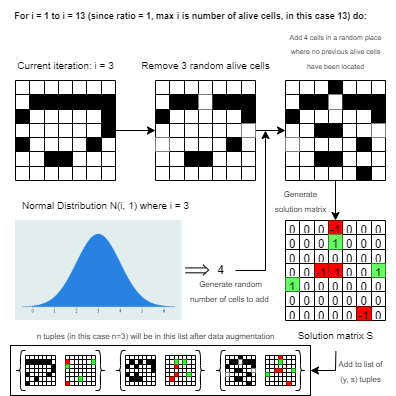
\includegraphics[width=1\linewidth]{dissertation/images/diagrams/data_augmentation_implementation.png}
\caption{Data augmentation from the HWSS. In this example, 3 sets are created for every number of cells removed. In this example, this will generate $13 \times 3 = 39$ augmented examples from 1 spaceship configuration.}
\label{fig:subim1}
\end{figure}

% However, the scoring network had additional data created for it. It was found that deconstruction data only did not have the best convergence. This was probably due to 

\subsection{Architecture of the networks}

\subsubsection{The probability network}

The probability network uses a series of convolutions and swish activation functions to find the given change of probability in a cell. The use of the convolutions is to encourage locality. In the GoL, only the cells in Moore's neighbourhood are considered (those directly adjacent). Therefore, it follows that a convolutional network would be the best fit, as the probability of a cell being present on a spaceship would largely depend on cells close to it. However, not only $3 \times 3$ filters were used. Near the end of the network, it was found that using $5 \times 5$ filters were very effective, which could be due to larger cell patterns depending on one another to fully move a ship. In between the $3 \times 3$ and $5 \times 5$ layers, a $1 \times 1$ layer was added. The argument behind this convolution is to modify individual cells which are more or less important based on where they are. This network was trained with the aforementioned "ratio deconstruction" method.

\begin{figure}[h]
\centering
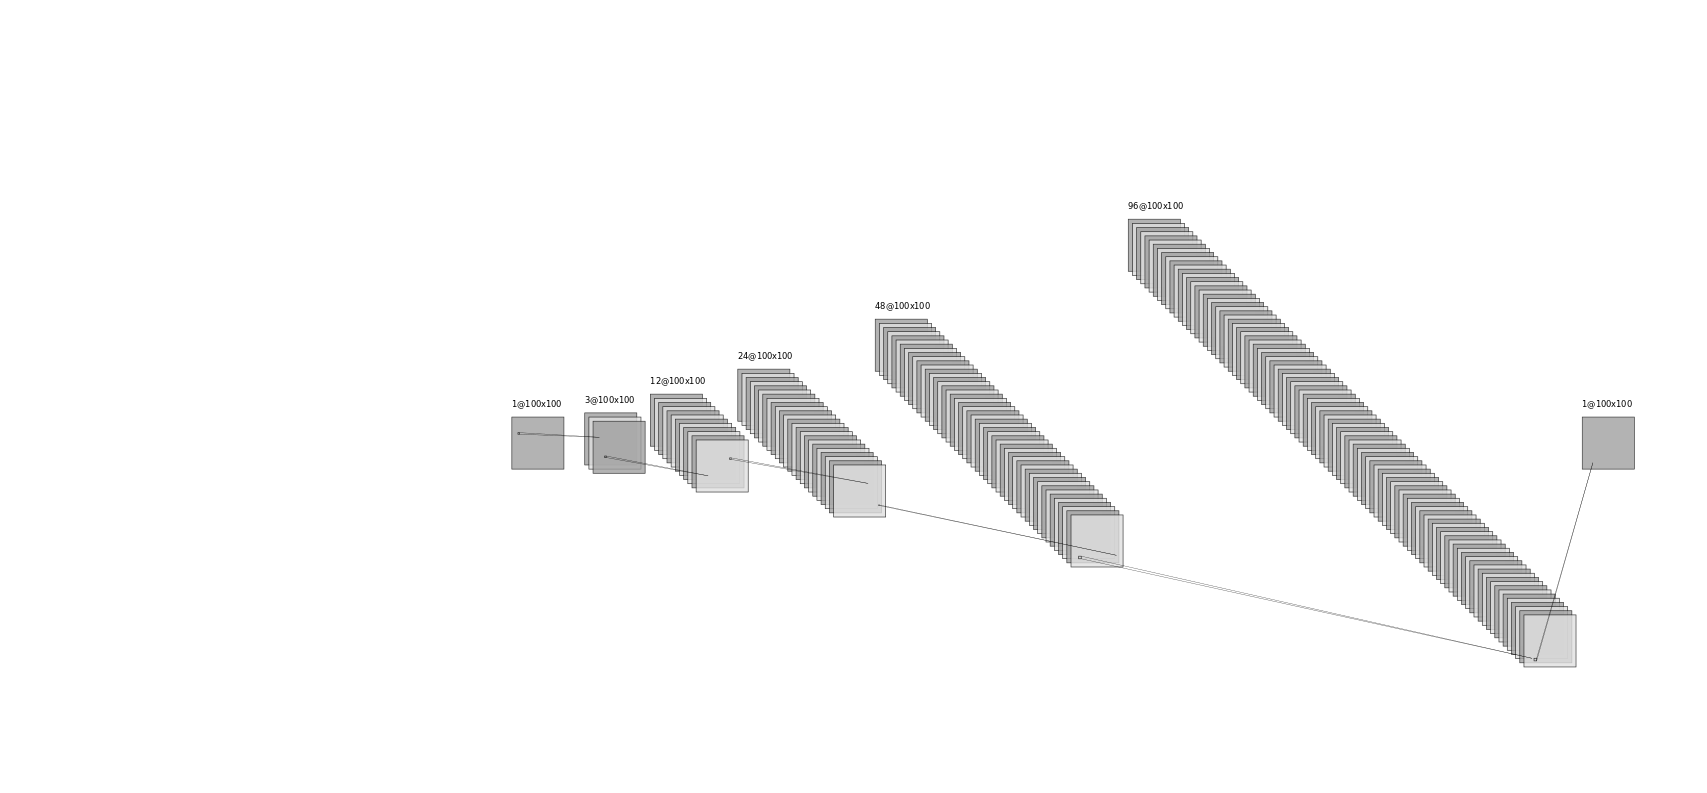
\includegraphics[width=0.8\linewidth]{dissertation/images/diagrams/probability_network_diagram.png}
\caption{Cell Probability change network}
\label{fig:subim1}
\end{figure}
\begin{figure}[h]
\centering
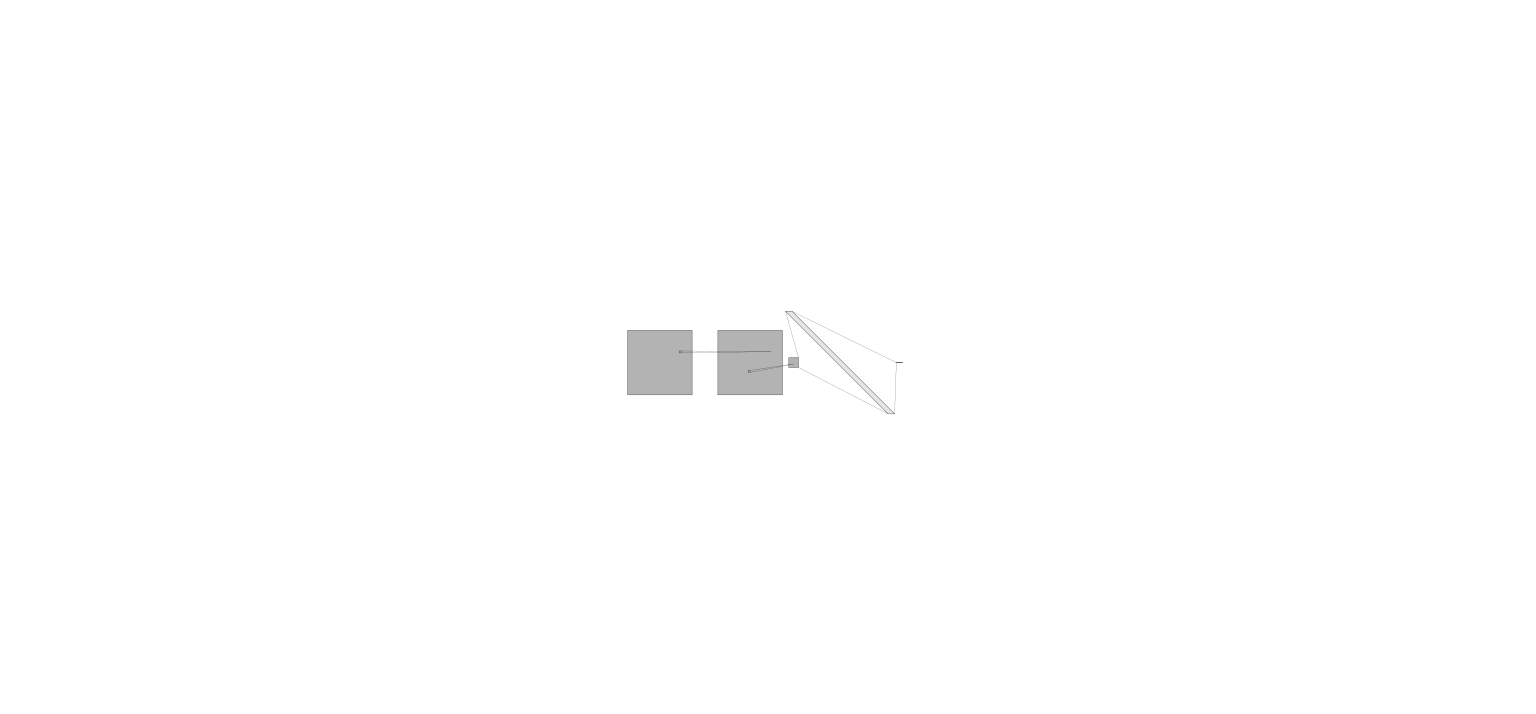
\includegraphics[width=0.8\linewidth]{dissertation/images/diagrams/scoring_network_diagram.png}
\caption{Scoring network architecture}
\label{fig:subim1}
\end{figure}

\subsubsection{The Scoring Network}

Using this probability network is good for finding potential cell changes given an input. However, it does not always give the best cell as a candidate. To decide which cells are the best, a scoring function is used in guiding search. The scoring network works in a similar manner to the probability network, with the exception of a average pooling layer before feeding the output into a fully connected network, which then outputs a score. This network also assumes that ships have a general underlying structure that can be detected by the convolutional network, and is different to the original ship probability function as it tries to model an existing function, and not a linear probability function. The goal of the network is to score structures that are close to being a spaceship higher, and to score structures that are further from being a spaceship lower. This was done by reflecting the resultant score on the $y$ axis.

Both the neural networks used an MSE loss criteria and an Adam optimizer based off torch. MSE loss was used as the criteria due to a difference of two matrices being well represented with such number. 

\subsection{The Searching Algorithm}

% \begin{algorithm}
% \caption{General Overview of the Search Algorithm}\label{alg:cap}
% \begin{algorithmic}

% \Procedure{search}{initialGrid}

% \State $currentNode \gets Node(initialGrid)$
% \State $n\_iterations \gets 5$
% \State $max\_depth \gets 30$
% \State $n\_considerations$
% \State $spaceships\_found \gets [..]$

% \For {i \gets 0 \to n\_iterations \do} {\State $bestNodes \gets [currentNode]$\; \For {j \gets 0 \to max\_depth \do} {\State $possibleActions \gets currentNode.getPossibleActions()$ \EndFor}\;
% \EndFor}

% \end{algorithmic}
% \end{algorithm}


\begin{algorithm}
    \DontPrintSemicolon
    \KwData{Implementation of the search function, $search(initialInput)$, which takes in an initial input grid. This grid must contain a few initial alive cells.}
        \KwResult{A list of spaceship data, in the form $[\{period, speed, rle\_code\}]$.}
    \Begin{
        $currentNode \gets initialInput$\;
        $n\_iterations \gets 5$\;
        $n\_tree\_returns \gets 5$\;
        $max\_depth \gets 30$\;
        $spaceships\_found \gets []$\;
        $i \gets 0$\; 
        \While{$i < n\_iterations$}
        {
            $bestNodes \gets []$\;
            $visitedNodes \gets \{\}$\;
            $j \gets 0$\;
            \While{$j < max\_depth$}
            {
                $possibleActions \gets currentNode.getActions()$\;
                $currentNode.incrementVisited()$\;
                add $currentNode$ to $visitedNodes$\;
                \eIf{\texttt{possibleActions not empty}}
                {
                    $currentNode \gets max(possibleActions, key: action.getScore())$\;
                }{
                    $currentNode \gets max(visitedNodes, key: action.getScore()$\;
                }
                \tcp{If the current node has a better score than the last node which was added to the list, then append it to said list.}
                \If{$currentNode.getScore > bestNodes[-1]$}
                {
                    append $currentNode$ to bestNodes\;
                }
            }
            $candidateNodes \gets bestNodes[bestNodes.size - n\_tree\_returns:]$ \tcp{Get top nodes}
            \ForEach{$node \in candidateNodes$}
            {
                \If{$checkSpaceship(node)$}
                {
                    append $getSpaceshipData(node)$ to $spaceships\_found$\;
                }
            } 
            \tcp{Now aggregate the nodes to find common values}
            $currentNode \gets aggregateCommonCells(candidateNodes)$\;
        }
        \Return spaceships\_found
    }
\end{algorithm}

[REMAKE THIS ENTIRE FIGURE]
\begin{figure}[h]
\centering
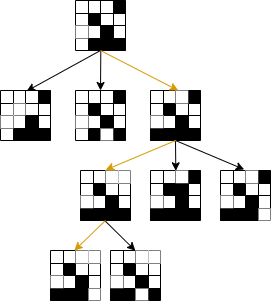
\includegraphics[width=0.8\linewidth]{dissertation/images/diagrams/tree_diagram.png}
\caption{Example of tree search to find the Glider. The most promising path is followed. Notice there are not always 3 candidates- that is because sometimes the number of cells that cross threshold values are below the maximum number of candidates.}
\label{fig:subim1}
\end{figure}

The search algorithm in this paper also works off a graph search, wherein different board states are represented as nodes, and each branch is a change in one item (cell), giving rise to a new board (state) with 1 different cell. This search is an A* approach to a tree formed by those nodes. The probability network is applied to the current state, and using fine-tuned threshold values, a select few of those cells are chosen to as branches to the current state node. The heuristic function of these nodes are calculated by using the scoring network. Once a node is visited, it is added to the "explored" list, with a visited attribute incremented. When the current state does not have any available nodes to expand into, for example if no cells in the probability change output surpass the threshold values set, then the state with the maximum score is selected from the explored list. This is the reason why the threshold values must be fine tuned: the tree search will keep moving down the tree as there will always be possible nodes to change without the threshold values. Furthermore, the threshold values are a function of the the current iteration in the tree, which means the restrictions on which cell to chose increases over time. The tree iteration method is done several times, and in between, a state aggregator is used to find the alive cells in common of the top $k$ items returned by the tree search. This gives a baseline model from which the tree search can be restarted, the idea being that only important cells would have been found by the top scoring states. The max\_depth value is also increased as the number of iterations increases. Iterating over a tree search is expensive, as it requires aggregating the states, but also checking if any of the returned states are a spaceship, which is difficult.


\begin{figure}[h!]
\centering
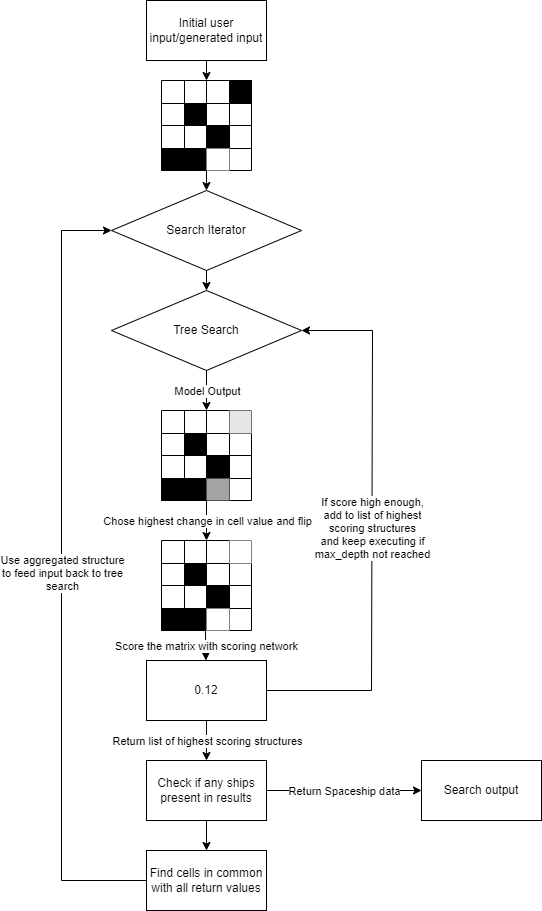
\includegraphics[width=0.9\linewidth, height=20cm]{dissertation/images/diagrams/gol_search_structure.png}
\caption{Search method architecture}
\label{fig:subim1}
\end{figure}

\subsection{Tree Search}

The search starts with an initial node $i$, set by the user or generated by the search program. This is then fed into the tree network as the initial state. The node is a class which contains a $getPossibleActions()$ method. $getPossibleActions()$ will return a list of candidate states (nodes) for that node, based firstly on the probability change network, and secondly by the threshold values. These threshold values are as follows:

The two threshold values are that of the removal of cells, and addition of cells. There are in total a maximum of 6 candidates, and a minimum of 0 candidates if no cells pass the threshold value. Once the cells that satisfy the threshold value requirements are selected, new nodes are created for those changes. States are evaluated by a the scoring network, and the number of times visited in this formula:
 
Once the next node has been selected, it is set as the current state, it's visitation count incremented, and added to the "explored" list. If there are no candidate states available to chose from, a node will be fetched from the explored list and set as the current node. The node that is selected is increased in number of times visited, and re-added to the list. The tree search will then continue, until max\_depth is reached, at which point it will return the top $k$ nodes with the highest scores. These are then checked for spaceships, and any relevant data is returned.

% MAKE THIS CLEARER
\subsection{Iterating over Tree Search}

\begin{figure}[h!]
\centering
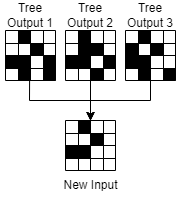
\includegraphics[width=0.4\linewidth]{dissertation/images/diagrams/iteration_aggregator.png}
\caption{The iteration aggregator in action. As can be seen, only cells in common are kept. The result is encouraging: only 1 cell away from the Glider. In this example, tree search outputs its top 3 highest scoring states}
\label{fig:subim1}
\end{figure}

[BIAS AJUSTMENT]

Although the tree search worked in some cases, a lot of the time the result of the tree search would be focused on one area of the tree which maximised the score, but did not find spaceships. This means that the solutions given were quite close to one another. To solve this problem, we needed a way to re-focus the search on the core parts of the ship. To to this, the top $k$ outputs of the tree search are aggregated in a way to only keep the cells in common. This is done with an AND operation over all outputs. When the tree search gets close to the solution, it has been observed that finding the correct cell which will fix the ship is difficult. This is most likely due to the scoring function: since MSE is a squared error function, the error is exponential in nature. When the algorithm comes close to converging to a solution, the change in score is almost insignificant. This leads the tree search to accidentally change the wrong cell, and therefore get stuck in a loop where it is essentially using trial and error to get the correct cell. By cutting the tree search at an early max\_depth, the input can be re-organised to (hopefully) only include the core cells important to the ship, and re-input them in the tree search. 

% IF YOU INCLUDE THE MAX_ITER BEING A FUNCTION INCLUDE IT HERE

Two major drawbacks of using this method is it may cut a solution early, and ship detection is slow. If the tree search is almost at the solution, then re-starting form the core cells may cause issues, as the program may get stuck in a loop of going down the same path, producing the same outputs, and therefore never creating a new output. Furthermore, ship detection is a costly operation, and by increasing the number of iterations, the speed of the algorithm slows down considerably.

\subsection{Other approaches for choosing next state}

There were 2 other methods thought about for choosing the next state. The first was to re-apply the network output on itself for a set amount of iterations. This, in theory, would create an output that would most resemble a spaceship in terms of what the network thinks will be the spaceship.

However, a major problem with this network is that the output is very negative (cell probability changes tend to be negative), which is due to the large amount of dead cells in any given spaceship. If the network output is re-applied to itself several times, information could be lost due to cell probabilities converging towards 0. This is why the branched cell-by-cell approach was selected: the probability does not converge toward 0, and the cell count can increase as well as decrease based on the output of the scoring function. Even if this problem were overcome, the network would face another issue: any input gives the same output. When the network is re-applied to itself, the model automatically normalizes the changes in probability. This then produces the exact same output on itself. A method to fix this may be to modify the training data to include floats as a solution, however the first problem of converging to 0 would still be present.

The second method is the greedy method, where the cell with the greatest change in probability is flipped, and used as input for iteration. This method completely disregards the scoring network and relies solely on the probability network, which could cause erratic behaviour. A major problem of greedy search is getting in a loop which is inescapable. For example, a loop could be created whereby the greatest change in cell value is a particular cell whether it is on or off, causing the tree search to continually flip the cell, preventing it from converging towards a solution. 


\section{Hyperparameter tuning}

\subsection{Model Parameters to Tune}

The following parameters were tuned, either manually or via early stoppage of the training program:
\begin{itemize}
    \item Learning rate
    \item Number of epochs
    \item Dataset size
\end{itemize}

The major difficulty with training a network to find new spaceships is avoiding overfitting. Overfitting in deep learning is when a network fits the training data very well, but does not perform as expected in a general scenario. This leads to program to only find existing ships, and prevents it from finding new ones. To mitigate this effect in the two different networks, early stopping was used. With this method, around 10 epochs were found to be optimal in training the neural networks. The learning rate was set quite low, 0,0005, as the model is very sensitive and therefore does not respond well to larger learning rate values. This value was found after some manual testing, as training took too long to optimally fine tune the learning rate.

The size of the dataset is an important factor, as a dataset which is too large may still overfit, even whilst controlling the number of epochs. Since all of the solution pairs are based off a small initial number of ships, it stands to reason that too many of said solution pairs will prevent the network from converging to a general point. To mitigate this issue, the network was trained on 20 solution pairs for every number of cells missing, which was found via manual testing, and hardware limitations (as increasing the number by 1 can add up to 50,000 solution pairs, significantly slowing down the training time).

\subsection{Algorithm Parameters to Tune}

There are a lot of parameters to the algorithm, which greatly affects the effectiveness of the search. Here are the notable ones:
 
\begin{itemize}
    \item $max\_depth$ : how deep should the tree go before ending a search iteration
    \item $n\_iterations$ : how many tree searches should be done with re-calibrated input
    \item $max\_n\_considerations$ : the maximum number of possible nodes that the tree search can pick from (maximum number child nodes any given node can have in the tree)
    \item $n\_tree\_returns$ : the number of grids returned by tree search which had the highest scores
    \item Threshold values : the threshold value for a cell to be considered as an candidate, to either be added or removed.
\end{itemize} 

\subsection{Tuning the threshold parameters}

The probability network has two main functions: to reduce the probability of a cell that is unlikely to be in a spaceship, and to increase the probability of a cell likely to be in a spaceship. This was tested by taking the mean increase in values. For cells that are not part of the spaceship (so called "undesirable cells"), the mean probability increase should be negative. For cells we want in the structure as they are part of a spaceship (desirable cells), the score should be positive. For cells which are not present in the structure and are not desired, the score should be close to 0. A similar value should be had for cells already present in the structure which should stay in the structure: there should be little to no change in probability. 

To find this graph, a set of ships were chosen, and incrementally, cells were removed from the ship. At the same time, extra cells were added, a similar method to the deconstruction method used in the data generation for training the neural networks.

\begin{itemize}
    \item Positive score: the mean value in desirable cells (the higher the better)
    \item Negative score: the mean value in undesirable cells (the lower the better)
    \item Intactness score: the mean value of cells in the structure that need to stay in the structure (the higher the better)
    \item Cohesion score: the mean value of cells added to the structure that need be removed (the lower the better)
\end{itemize}

\begin{figure}[h!]
\centering
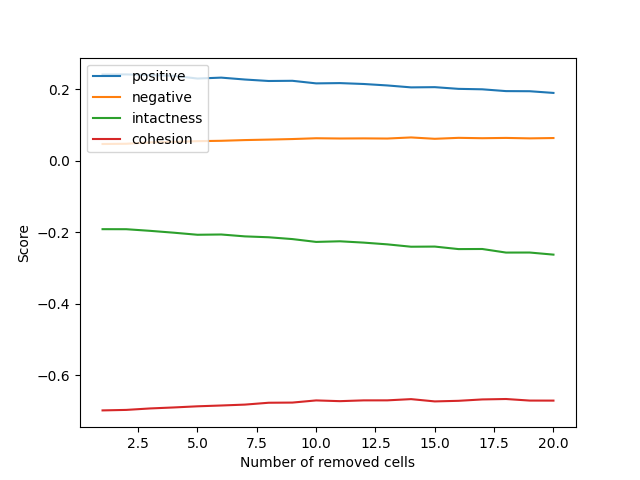
\includegraphics[width=0.8\linewidth]{dissertation/images/graphs/n_removed_cells_score_probability_analysis.png}
\caption{Mean scores for positive, negative, intactness and cohesion on different ships. On the x axis, the number of removed cells is represented. On the y axis, the average score the network assigned to a group of cells is displayed. Ideally, the 'positive' and 'intactness' line would be close to 1, and the 'negative' and 'cohesion' line be close to -1}
\label{fig:subim1}
\end{figure}

As can be seen by the graph in Fig 4.9, the results are mixed. Although the positive value is high, it is quite close to the negative value. Ideally, the negative score line would've shifted far into the negatives, however it is positive in value, meaning that applying the probability change network on itself would, on average, increase the probability of cells which should not be present. The intactness score is also low. In an ideal scenario, the intactness score would be at the very least above 0: cells already part of the ship should not be removed. Finally, the cohesion score is quite good: the value is on average very negative, meaning cells which are not supposed to be present are being removed by the model network. From this graph, we can extract some of the tuning parameters: an upper bound threshold of 0.15, and a lower bound of -0.6.

However, these threshold values can be improved upon. By making them dynamic, the deeper the search gets, the more the thresholds increase in size. This is done for two reasons: to weed out cells which are irrelevant the closer you get to a ship, and to allow nodes already explored to be re-explored. The "explored" list is only used when there are no candidate cells given a state, so by increasing the threshold values, the number of candidates go down and allow for other paths to be visited. The formula for those computations are as follows:

\[ upper\_bound = upper\_bound + (\frac{current\_iteration}{max\_depth} \times  0.1)\]
\[ lower\_bound = lower\_bound - (\frac{current\_iteration}{max\_depth} \times  0.1) \]

Where $current\_iteration$ is the $i^{th}$ iteration in the tree search sequence. These equations were found as optimal after testing. These values allow only a max upper bound of $u \leq 0.25$ and a minimum lower bound of $l \geq -0.7$, which prevents the bounds from being unreachable by candidate cells. Due to this, the tree search can still find new candidates, however will encourage the search to go back to previous results. more often at the end of the search.

Applying the network to see the extrapolated cell counts after the threshold are set is equally important in determining the efficiency of the model inside the search algorithm. In Fig 4.10, the number of cells that have been added to the network which are not part of the spaceship, and the number of cells added which are part of the ship are shown. As can be seen from the graph, the number of cells missing is quite low, with about half of the initial cells missing having been recovered. However, the number of extra cells is quite significant. These extra cell counts can be explained in Fig 6.3. This graph shows the average score of the extra cells: they are very positive, to the point where the probability surpasses the threshold. On the flip side, the missing cells have a very negative value. This leads to cell probabilities being in the wrong threshold values, and the wrong cells being flipped. The only solution to this is to re-train the probability change network into giving more accurate predictions on cell probability changes.

\begin{figure}[h!]
\centering
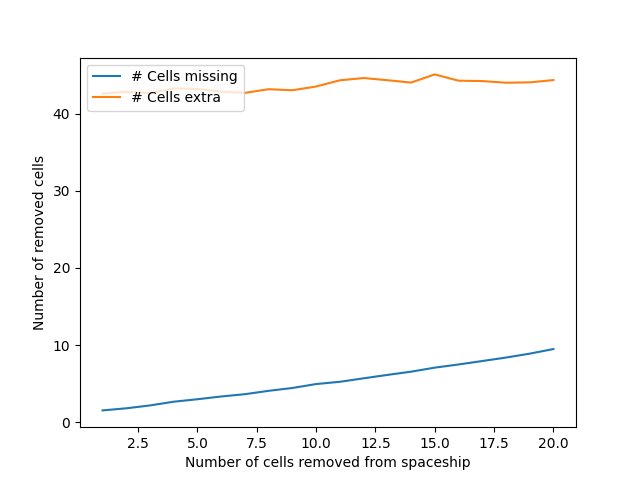
\includegraphics[width=0.8\linewidth]{dissertation/images/graphs/cells_removed_n_cells_extra_missing_probability_analysis.png}
\caption{Number of removed cells compared to number of cells missing/extra after extrapolating a new grid using pure network outputs and the set threshold values. In an ideal scenario, both lines would be as close to 0 as possible.}
\label{fig:subim1}
\end{figure}

\begin{figure}[h!]
\centering
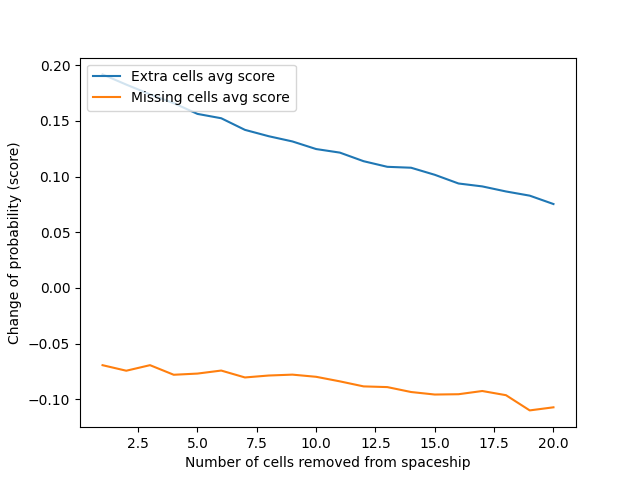
\includegraphics[width=0.8\linewidth]{dissertation/images/graphs/cells_added_n_cells_extra_missing_probability_score_analysis.png}
\caption{Number of removed cells compared to the average score of cells missing/extra. The missing cells are negative (we want them to be as positive as possible), and the extra cells are high in probability (we want them to be as negative as possible)}
\label{fig:subim1}
\end{figure}

\subsection{Tuning the other parameters}

The number of iterations, number of cells considered, and the max depth are also important factors. If there is a higher number of cells considered, then there will be a greater number of branches in any given node, which makes the program slower. However, it may find a branch with a higher score, which could increase the performance of the search. Similarly, a higher max depth value will lead to a more thorough search of a start configuration, but it will make the program slow, and may lead the program into a state in which it can no longer improve. Another consideration to choosing the max depth is the initial state. If the user is looking for new ships, then they will only start with a few concrete cells. This means a high max depth is needed to fill in the empty cells. However, if repairing a ship, a lower max depth may be beneficial in order not to skew too far from the ship structure. The number of iterations has less of a trade off. The more iterations there are, the higher the likelihood of finding the ship. However, to keep the algorithm short, a small testing value was used. In the end, the following parameters were set:

\[ max\_n\_considerations = 3\]
\[ max\_depth = 30\]
\[ n\_iterations = 3\]


\section{Tools Created and Used}

\subsection{RLE Encoding}

Since storing a GoL matrix is quite expensive, a compression method is used to store structures. It is a type of run length encoding (RLE), which denotes the cells that are alive. It is used a lot when generating training data for the different networks. The encoding takes place over two lines, with one containing the size of the structure, and the next one being the actual token encoding method. The first line is represented by: $x = n, y = n $ such that the structure is of size $n \times m$, width and height respectively.

The tokens used in this encoding are as follows:

\begin{itemize}
    \item $b$ : dead cell
    \item $o$ : alive cell
    \item $\$$ : end of line
\end{itemize}

Every token is represented by a number before the token. If there are $n$ alive cells in a row, it is represented as $no$. If a cell does not appear consecutively, there is no number associated with that token. For example, an interweaving of dead and alive cells on a single line would be represented as $obobobob$ and so on. After the last alive cell, the dead cells are not encoded into the RLE code, this is assumed automatically. If there are $n$ empty lines in a row, then the empty lines are denoted as $n\$$. An example RLE is of the glider: \newline $x=3,y=3 \newline bo$2o$obo!$
% RE-FORMAT THIS MAYBE ? THE RLE CODING 

% TALK ABOUT HOW RLE VALUES HAD TO BE EXTRACTED AND PROCESSED
% DO I TALK ABOUT THIS?
The RLE values for spaceships used in the ship search were stored in a text file which needed to be extracted and processed when training, validating, or testing data.

\subsection{The Game of Life}

To execute some parts of the program, such as the spaceship check method, a GoL implementation was needed. There are some existing tools in python to run the GoL, namely "Golly", which is used in some python search algorithms like "gfind". The use of Golly was considered in the project, however its lack of versatility, poor documentation, and difficulty in adding test code led to the decision of creating an independent GoL tool using numpy. This allowed great leverage of the code, and made different kinds of step-by-step analyses easier to manage. The cells are represented in an $n \times m$ numpy matrix, and every time step a neighbour matrix is applied to find the number of neighbours of an individual cell. With this information, the rules of the GoL can be applied, and a new matrix representing the next time step is produced. 

Inside of this GoL implementation, several sub-tools were produced, such as:
\begin{itemize}
    \item A function to return the next time step, or the state after $t$ time steps 
    \item Representation of the current board using Pygame / matplotlib
    \item Ship data calculator: extracts the speed, size, and general properties of a structure
    \item Structure manipulations: normalizing a structure to fit the RLE encoding, extracting a structure from noise, putting a structure into a sandbox (empty grid) environment
\end{itemize}

These methods were used at various points, from training the networks, to analytics. Further modifications of the GoL code allowed structure data (such as average neighbours, average number of cells over time, changes in cell values) to be extracted, which could not be done with Golly. 

\subsection{Determining if a structure is a ship}

% WRITE ABOUT HOW THE SPEED OF THE SHIP IS CALCULATED
This process was used in a relatively straightforward manner. First, a maximum period search time is defined, $p$. This value will be the maximum period a found spaceship can have, which is used to prevent a structure from evolving forever. The idea is to take the structure, place it in an expanded empty grid, and evolve it until it has reached its initial state. The main drawback of this method is that ships which have a period above $p$ will not be detected. Furthermore, this approach is inherently slow: with $p$ iterations and $n$ spaceships needed to be checked, it is quite heavy on the search. Furthermore, larger cell structures take more time to check, as they need a larger grid. This value is also variable. For a larger search, a larger amount of space is needed to allow the ship to oscillate properly. For $100 \times \100$ search grid, a padding of 150 cells is needed in each direction in order to properly assert that a structure is indeed a ship. Therefore, a function to determine the search size needs to be formulated, which can depend on the spaceship, given some expand a great deal before contracting into their original shape again. In this search algorithm, a padding size of $padding = 150$ was used as a default. However, it is recommended that the padding size be of the form $padding = max(w, h) \times 1.5$ where $w$ and $h$ are width and height respectively.

\subsection{Analytical Tools}

The tools build to test the different networks and the search algorithm were extensive. As seen previously in figures 4.7, 4.8 and 4.9, a lot of analysis was done on different cell removal values. However, more analyses were done on max\_depth values, and iteration counts, which were used to generally test the algorithm and figure out some useful values. These tools worked quite simply by iterating over several lists of possible parameter values, and recording them in a pandas table.  Data processing using pandas' aggregator function was used to collect relevant data, and matplotlib was then used to display these results in a useful fashion. 

Three main tools were used to test the algorithm: the probability change network tests, the scoring network tests, and the search algorithm tests. These were implemented as 3 separate functions, which ran when a new model was trained. A grid CV search method was used in each of these methods to get optimal values. Every test value is iterated over to find the best, and produce graphs to display the efficiency of the algorithm. The probability change network relied on the scoring graph such as the one in Fig 4.7, and was the most efficient way to test the efficacy of the network. Testing the scoring network was quite easy, as different structures were tried to correlate the score. This made it extremely quick, and easier to fine-tune compared to the probability change network and the search algorithm. As for algorithm itself, tests had to be run on a smaller subset due to the time taken for a single execution. All the results of tree search were returned, and an average is taken over those results. An important metric is the probability of reconstruction, which involved running the algorithm on a set of cells with missing ships. The deconstruction tool helped in creating ships with this deconstruction: by removing a number of cells $n$ and adding a few random ones, just like in $ratioDeconstruct$ which was used in the data augmentation.


\subsection{Summary}

In this chapter, we looked at the techniques and technologies we used to develop the search method, which included a whole host of python programs like numpy, pandas, matplotlib, and general work methods used to plan development. This was then followed by previous attempts to solve the problem, such as the ship probability method and stochastic ship cell probability, along with their shortcomings. For example, ship probability not being granular enough, and the convergence issues of a stochastic search. In the challenges section, we go over the major difficulties of the problem, such as NP hardness, slow convergence of networks, large amounts of data, and no previous work done on the subject. The probability search section went into detail about the two networks used (the probability change network and the scoring function), and how they are used in the tree search algorithm. This algorithm was described in detail, describing a type of A* search method, along with the iteration over the the tree search being beneficial to reaching a solution. In the tuning section, we go over the important threshold values to deciding if a cell should be set or not given the output of the probability change network, and how we fine tuned it. Equations are given as to how to make these values dynamic depending on the current iteration or depth of the search. Finally, the tools section goes over important scripts that were used to build the program, as well as analyse it, such as RLE readers, GoL implementations, and analytical tooling.


%==================================================================================================================================
\chapter{Evaluation} 

\section{Aims}

The main question to answer in this paper: does using neural networks in a tree search of spaceships work in practice? Success in this measure would mean at the very least converging to a known solution which has not been seen by a neural network. This would entail removing cells from a spaceship which has not been trained on, and reconstructing the original ship through the search. This should be done in a way that beats random selection of cells. However, it is also not a binary metric: the performance is to be measured on a range of missing/extra cells. If the number of missing cells from the ship is high, and the algorithm can still reconstruct the original ship, then it is a sign it is performing well. An even better metric would be to find a spaceship that has not been found as of yet.

Another question that would be greatly beneficial to answer would be that of the main assumption: is there a general pattern to spaceships that can be found using a neural network? Success in this domain is harder to define. If a the probability change network is consistently scoring the next cells to be placed correctly, then it would be a measure of success. If the scoring network is correlating close to the MSE (Mean Squared Error) of a spaceships with cells missing, then this also may prove that the network has learned a general pattern to said ships.

\section{Methodology}

The experiments were run via a singular analytics script, which went through every metric devised. These values were stored in a table of results aided by pandas, and then graphed with matplotlib. This analytics program was ran every time a change to the network was made, or to manually tune parameters. Furthermore, the script is compartmentalized into metrics for the two different networks and the algorithm as a whole. This allowed for tuning using a grid search to find the optimal parameters, notably the threshold values.

To keep the experiments on different values fair, the following variables were set to be constant:
\begin{itemize}
    \item max\_n\_considerations: number of branch nodes for any given node, set to 3
    \item max\_depth: max depth of tree search, set to 30.
    \item n\_iterations: number of iterations over tree search, set to 3.
    \item n\_tree\_returns: number of best grids found by tree search, set to 5.
\end{itemize}

Said values were found by manual trial and error of the algorithm. This was set manually as searching for the optimal values was impossible given the hardware available. Another aspect to note is the number of iterations, which was set to 3 for similar reasons. Although the number of iterations being set to a higher value would almost guarantee better results, the algorithm is costly and restrictions needed to be set due to the time limit of this project.

The following independent variables were used as testing metrics:
\begin{itemize}
    \item Number of distinct ships tested on: 50
    \item Spaceship types: seen or unseen (spaceships that have been trained on, and spaceships that are used for testing)
    \item Number of cells removed: from 0 cells removed to 50.
\end{itemize}

These were set to standardize the results for any given testing metrics. Fifty spaceships is enough to get a reliable trend on the data, allowing for smooth curves and trends to be found. A noticeable variable is the number of cells removed. 50 cells is enough to completely delete a spaceship from the grid, and replace all of the cells with random ones. This is intentional, as it tests the ability of the search to work from scratch.

Dependent variables used for measuring the performance of the two different neural networks and the search algorithm as a whole:
\begin{itemize}
    \item The average score (probability increase/decrease) in a given group of cells
    \item The number of extra/missing cells in a spaceship after applying the threshold values 
    \item The average score of extra/missing cells after applying threshold values
    \item The MSE (Mean Squared Error) between a resulting grid and the target spaceship 
    \item The number of spaceships that were found for any amount of missing cells
\end{itemize}

These metrics will give a good idea of performance as a whole. The scoring network, for example, will only be measured via the MSE metric, since it is trying to correlate a score to said metric. However, the search algorithm can be measured by the number of spaceships found, average score of extra/missing cells, and the number of extra/missing cells. Other values were experimented with, for example the average MSE of algorithm results compared to the original ship deconstructed, however these performance results proved less indicative than those listed above.

\section{Results}

\subsection{Probability Network Performance}

Although the probability network worked decently with training data, it had severe limitations when used on unseen test data. Using training data, scoring results are outlined in Fig 4.x. In this graph, you can clearly see the tends: a high value for desired cells, undesirable cells have a lower score. However, on untrained data, the results were less positive. The network remains good at removing "undesirable" cells which have been added by the search algorithm, however the "desirable" cell scores have dropped drastically, as well as the intactness score. These trends indicate that the probability network has generalized poorly. Without these high positive values, it is very hard for the network to correctly predict which cells are the best candidates. It is easy for the network to make mistakes. As seen later in the evaluation of the entire algorithm, the probability network on the test data greatly affects the performance of the search in a negative way. From these results, it is highly unlikely that the network has found a general pattern to spaceships. Although the cohesion score seems encouraging, the network is inherently negative. This means it is good at removing some cells which have been added that should not be there. However, the undesirable cells are still high in value. This implies that cells not supposed to be there will still appear. This evidence is further supported in Fig 5.x, where a clear number of extra cells can be seen. This is almost double the average of the trained ships, which indicates further failure to generalize, Furthermore, the number of missing cells stays near constant - which on the surface level may look like a good thing, but is more likely due to random chance instead. 

% do i include missing/extra cell scores?

\begin{figure}[h!]
\centering
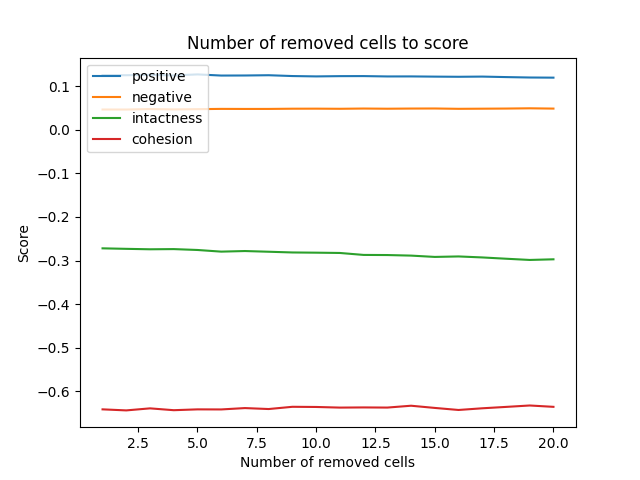
\includegraphics[width=0.7\linewidth]{dissertation/images/graphs/n_removed_cells_score_probability_analysis_test.png}
\caption{The probability scores for untrained data. It is mostly the same, however the positive scores are even lower on the graph. This is bad, although by re-tuning the threshold it is possible to increase the efficiency of the search on untrained data.}
\label{fig:subim1}
\end{figure}


\subsection{Scoring Network Performance}

The entire objective of the scoring network is to best approximate the MSE function from a structure to a spaceship. The output of the scoring function is an increasing value as it gets closer to the ship. However, the actual MSE approaches 0 as the structure gets closer to the ship. To best represent correlation between the two, the axis in this example has been flipped on $y = 0.08$. Measuring the effectiveness of the scoring network was easy: just try removing cells from the ship and testing to see the network output.
% maybe add the original scoring function here

 The results on the test dataset yielded good scores. As can be seen in Fig 5.2, there is a clear correlation between the true MSE and the predicted MSE. This could potentially imply that the main assumption of  a general structure being present in spaceships is true. Furthermore, a direct correlation is not exactly necessary. Since the objective of the scoring function is to direct the search to a solution, the main feature needed is a downward correlation between distance from structure and a potential ship. However, it remains to be seen what exactly causes this MSE to work as well as it does. It could be due to a particular density of alive cells in a certain area being more likely to be a spaceship, and not the actual form of the structure itself. To test this, we used the deconstruction method to add random cells in the structure where dead cells are supposed to be, keeping the density at a similar level. As can be seen in Fig 5.2, this correlation was still present given these extra cells, indicating that the network may be functional.

 % should I test this scoring network by giving it all cells as an option and see if it picks correct one?
 

\begin{figure}[h!]
\centering
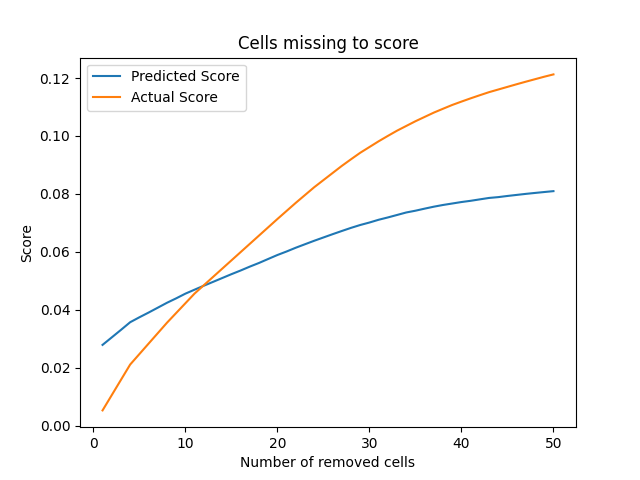
\includegraphics[width=0.8\linewidth]{dissertation/images/graphs/cells_missing_to_score_trained.png}
\caption{Number of removed cells to score for trained ships}
\label{fig:subim1}
\end{figure}

\begin{figure}[h!]
\centering
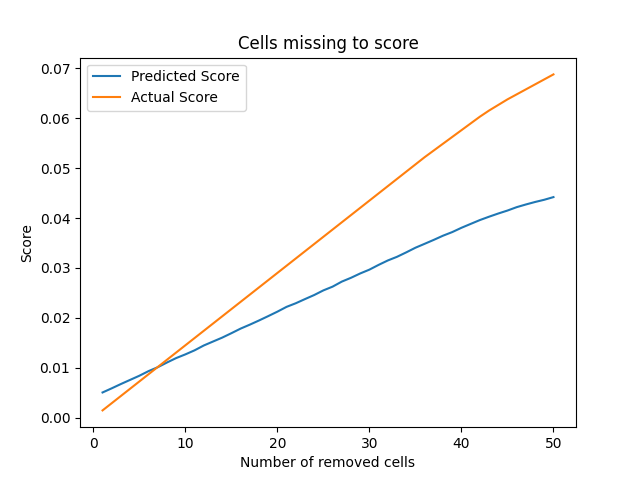
\includegraphics[width=0.8\linewidth]{dissertation/images/graphs/cells_missing_to_score_test.png}
\caption{Number of removed cells to score for untrained ships. The predicted score and actual score correlate well.}
\label{fig:subim1}
\end{figure}

\subsection{Search Performance}

% TALK ABOUT TESTING ON AN EMPTY / VERY SPARSELY POPULATED GRID TO CHECK THE PERFORMANCE

The outputs of the search could be manipulated in several ways to produce evaluation metrics. Most of them also revolve around the idea of "missing" and "extra" cells after the program has finished executing. The metrics are taken from the top $k$ boards at every iteration which are returned after tree search, and are averaged by number of missing cells. The MSE of the structure is also calculated, along with the reconstruction chance, which is calculated by taking the number of times a spaceship was found over the total amount of times tree search was run.

% SHOULD I INCLUDE THE PARAMETER TUNING STUFF?

\begin{itemize}
    \item The number of cells missing: number of desirable cells not part of the structure
    \item The number of cells extra: number of undesirable cells
    \item The MSE score from to the target spaceship
    \item The chance of reconstruction given number of cells missing from original ship
\end{itemize}

However to truly test if the algorithm is performing well, the best metric is the chance of reconstruction given a number of cells missing. Results from running the algorithm on a test dataset are disappointing. The probability of ship reconstruction is virtually 0 for any ship that has not originally been trained on, as can be seen in Fig 5.3.

\begin{figure}[h!]
\centering
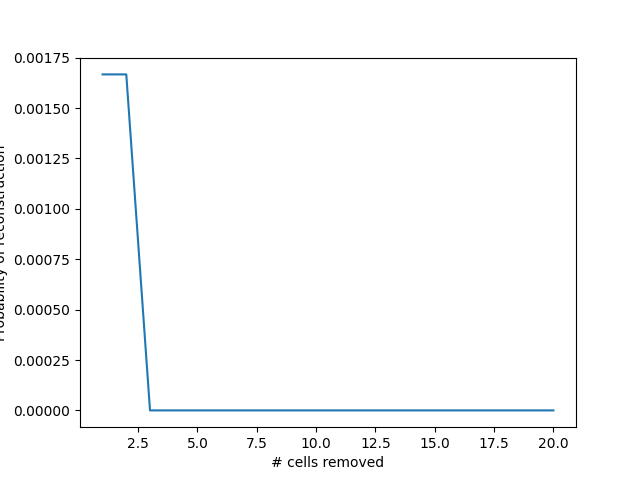
\includegraphics[width=0.8\linewidth]{dissertation/images/graphs/probability_of_reconstruction_against_damage_testin_only.png}
\caption{Number of removed cells to probability of reconstruction for untrained ships (ships that were not used in training the networks)}
\label{fig:subim1}
\end{figure}

A failure in the probability change algorithm is the most probable contender for the poor results, which are most likely due to overfitting of the network. Being that there are so few ships to begin with, and the network takes a long time to converge, this is somewhat unsurprising. However, reconstruction probability from trained ships is higher. Although not useful to finding new ships, this does point to the possibility that the search algorithm may work if a better trained network is used. The results of reconstruction are outlined in Fig 5.3. Another potential issue is the tree search itself. Given the issue of computing power, optimal parameters were not thoroughly tested for the number of considerations, or for the number of best states returned by the tree search. These are parameters that could greatly change the outcome of the search algorithm. To determine the optimal parameters, more grid search would have to be performed, however it was not feasible given the hardware used in this paper. 

%is this better than a random algorithm? Maybe. Is there a way to test?

\begin{figure}[h!]
\centering
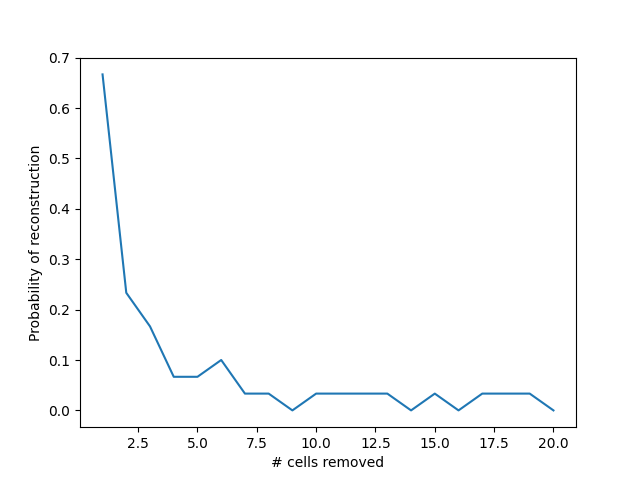
\includegraphics[width=0.8\linewidth]{dissertation/images/graphs/probability_of_reconstruction_against_damage_trained.png}
\caption{Number of removed cells to probability of reconstruction for trained ships (ships that were used in training the networks)}
\label{fig:subim1}
\end{figure}


\subsection{Average Iteration Convergence}

- here input results of how many iterations to a spaceship


\subsection{Comparing Search the Algorithm with Existing Ones}

It is quite hard to compare the performance of this search algorithm with others, given how different they are. 

- ikpx algorithm
- gfind
- other algorithms which could fit

\section{Discussion}

From the following results and observations, it is clear that the network did not work as hoped. There are a variety of problems plaguing the algorithm, but the main one is the probability change network. The search problem is inherently deterministic, and one small change in a cell can either make or break a spaceship. Due to this nature, a convolutional network may not be the most suitable, as it is prone to noise. Furthermore, since the entire role of the probability change network is to find the best candidate cells to finding a new ship, the entire search relies on it. As seen in section 5.1.1, the network woefully under performs in this aspect when fed unseen test data. This may be due to overfitting the spaceship patterns, as there may not have been enough variety in the data to find a general pattern to spaceships. However, without extensive training on the data, the network was virtually unable to converge. Given this fact, it is probable that the network has simply learned the known spaceship structures. On the other hand, it is possible that there is no general pattern to spaceships. The network failing to converge may be proof of this: if there were a pattern, there would be a convergence earlier on without the need to overfit. This paper has neither proven nor disproved the existence of such a structure. Given the results of the scoring network, it is possible such a pattern exists, due to the correlation between the true MSE and the predicted MSE, however more testing must be done to prove it in a conclusive manner. In addition, the scoring network may still be the key to finding spaceships with neural networks. If a logical method was used to find candidate cells, instead of the probability change network, the scoring heuristic function could still guide the search. Proper testing for this would involve giving the network the correct cell as an option, and checking to see if the scoring network can correctly predict which cell was the best out of a range of options.

Given all these issues, it would be easy to brush off this search algorithm as a failure. But there is still use to it. For example, the network converges quicker than logical algorithms in grids above a size of $20 \times 20$. In a typical logical search algorithm, it would take a lot of time for the search to reach higher levels, such as $100 \times 100$ grids. Using the probability network, it is possible to quickly reach a set of cells which might contain a spaceship, even though a final working structure is not found. If combined with a typical logical search, it may be possible to improve the algorithm into finding correct, large, ships.

\section{Summary}

The main objective of being able to converge on new spaceships was not reached. The search algorithm found very few spaceships that it was not trained on, and only those which are missing 2 cells. This is better than a random search, but is still not enough proof to ascertain that the algorithm is working as intended. Furthermore, after running the network on some starter configurations, no new spaceships were found. However, there are some promising findings. The scoring network worked much better than anticipated, correlating almost perfectly with the actual mean squared error of ships it was tried on. This does not prove the the assumption that spaceships have a general pattern, however it does pave the way for future progress. It is still an open question whether or not the scoring network has properly learned to score a potential spaceship, or if it has learned another feature, such as the density in the area where a spaceship should be. To determine this, more neural networks would need to be trained and tested.


%==================================================================================================================================

\chapter{Conclusion}    

\section{Conclusion}

The use of neural networks in the game of life still has a long way to go. A lot of the questions posed in this paper remain unanswered, and have raised yet more of them: will a UNet work better? Is accelerating tree search the optimal way to use neural networks in the GoL, or is there a way to skip this step? Can neural networks even be used in the GoL? However, it is clear that the algorithm has potential. Although there are many improvements to be made, the fact that the scoring function worked so well, that ships can be reconstructed quickly with large amount of cells missing, means that the search isn't totally random. Generalization is by far the most important aspect to look at in the future, either by using more spaceships, using a different network, or more powerful machines which can run proper hyperparameter tuning programs.

The data augmentation, from expanding one ship into many, to using a deconstruction method to create many solution datasets, has many advantages and disadvantages. For starters, it can easily create a large dataset out of very few ships. This is good, as data on the GoL is sparse in general, therefore being able to expand the dataset in this manner is a great improvement. However, there remain issues with this approach. Since the initial dataset is so small, it remains to be seen if a pattern to spaceships can be derived from only those base spaceships. Deriving all the augmented data from this initial dataset leads to severe overfitting of the initial data, seriously harming the performance of the network on unseen data.

The probability change network was designed in a convolutional manner, as the game of life has locality inherently present in its system. These convolutions used $3 \times 3$ and $5 \times 5$ convolutions, which were chosen after tying out a set of different values. Although the network proved it could predict cells on trained data, it failed to do so more generally. Regardless of this, it shows that an approach involving locality is effective compared to a fully connected network, which makes sense. It may be that more/less convolutions could bring about better results, however this is yet to be tested. A different approach to the convolutions, for example a UNet, or a similar denoiser network, may be more effective. Furthermore, the opposite operation could be done: start with a grid of cells all alive, and remove those which are not useful to a ship. Although this was trained in the network, it could be more efficient, [FIX THIS YOU KNOW WHAT I MEAN]

The final search tree method worked by selecting a number of candidates using the probability change network (selecting the greatest changes of value above a certain threshold), and checking the improvement of those changes using the scoring network. This had the effect of creating a search similar to A*, as the scoring network can be seen as a heuristic function to searching the graph. When the tree search has reached its max depth, it returns the top $k$ nodes with the highest scores, which get aggregated in a way that retains only the cells in common, and is then re-fed to the tree search. However, due to the lack of speedy hardware, and therefore parameter tuning, there are a lot of factors that can be improved on. For example, the number of candidate cells to change is an important factor in a speed-efficacy trade off. The number of grids returned by tree search could also be tuned to best fit the aggregation of the tree search results.


\section{Future Work}

Using a neural network for spaceship search in the future is likely to give some promising results if the network is based off a denoiser. In recent years, these networks have been incredibly effective in creating sharp images using context \cite{Zamir_2022_CVPR}. If these networks could be trained in a way that could find spaceships, and the general spaceship pattern hypothesis is true, then there is a lot of potential. Furthermore, adding a logic based spaceship search after the output of the neural network based search may yield interesting results. Since it was seen that the network can quickly find large structures, a logic search based off this output may find new ships. However, this still depends on the general spaceship hypothesis, and a new network may need to be trained to specifically target this task.

As a final note, using a network to predict the shape of a spaceship may not be the only way to solve this problem. Another interesting approach would be to train a network, such as the scoring network, to find the "utility" of a pattern. A genetic algorithm could then be evolved to maximize this utility function, which could be to find spaceships with a certain property (size, speed, period). This method may have more base data to work with, and as seen with the scoring network results in this paper, may have potential to work.


%==================================================================================================================================
%
% 
%==================================================================================================================================
%  APPENDICES  

\begin{appendices}

\chapter{Appendices}

Typical inclusions in the appendices are:

\begin{itemize}
\item
  Copies of ethics approvals (required if obtained)
\item
  Copies of questionnaires etc. used to gather data from subjects.
\item
  Extensive tables or figures that are too bulky to fit in the main body of
  the report, particularly ones that are repetitive and summarised in the body.

\item Outline of the source code (e.g. directory structure), or other architecture documentation like class diagrams.

\item User manuals, and any guides to starting/running the software.

\end{itemize}

\textbf{Don't include your source code in the appendices}. It will be
submitted separately.

\end{appendices}

%==================================================================================================================================
%   BIBLIOGRAPHY   

% The bibliography style is abbrvnat
% The bibliography always appears last, after the appendices.

\bibliographystyle{abbrvnat}

\bibliography{l4proj}

\end{document}
